\begin{enumerate}
  \item Pour $k\geq 1$, on peut {\'e}crire
\begin{displaymath}
 (k+1)\binom{n}{k} = k \binom{n}{k} + \binom{n}{k} = n \binom{n-1}{k-1} + \binom{n}{k} 
\end{displaymath}
d'o{\`u} , en notant $S$ la somme cherch{\'e}e :
\begin{displaymath}
 S=n\sum_{k=1}^n\binom{n-1}{k-1}+\sum_{k=0}^n\binom{n}{k}= n2^{n-1}+2^n = (n+2)2^{n-1}
\end{displaymath}
Autre solution. Consid{\'e}rons la fonction $f$ définie par $f(x)=x(1+x)^n$. Alors $S=f'(1)$ or $f'(x)=(1+x)^n+nx(1+x)^{n-1}$ d'où $S=2^n+n2^{n-1}$.

\item Factorisons la différence. 
\begin{multline*}
  (m+2)x+1 - \frac{1+x+x^2}{1-x} = \frac{(m+2)x+1-(m+2)x^2 -x-1-x-x^2}{1-x}\\
  = \frac{mx-(m+3)x^2}{1-x} = \frac{\left((m+3)x-m \right)x }{x-1}
\end{multline*}
L'in{\'e}quation propos{\'e}e est {\'e}quivalente (pour $m\neq -3$) {\`a}
\begin{displaymath}
 \frac{m+3}{x-1}x(x-h(m))<0 \text{ avec } h(m)=\frac{m}{m+3}= 1-\frac{3}{m+3}
\end{displaymath}
\begin{figure}[h!t]
 \centering
 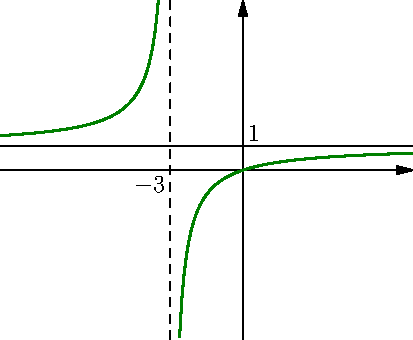
\includegraphics{./Celem5_1.pdf}
 \caption{Graphe de $h$}
 \label{fig:Celem5_1}
\end{figure}
Le signe de cette expression est facile à évaluer pour $x$ plus grand que $0, 1, h(m)$ et elle change de signe en chacune de ces valeurs. On doit donc classer 0, 1, $h(m)$ suivant $m$ en étudiant le graphe de $h$ qui est une hyperbole. (fig \ref{fig:Celem5_1}). On obtient:
\begin{itemize}
  \item Si $m < -3$,
\begin{displaymath}
0 < 1 < h(m)\hspace{0.5cm}\Rightarrow \hspace{0.5cm} \mathcal{S}_m = \,]0,1[\, \cup \, ]\frac{m}{m+3},+\infty[  
\end{displaymath}

  \item Si $m=-3$, l'inéquation devient
\begin{displaymath}
  \frac{3x}{x-1}<0  \hspace{0.5cm}\Rightarrow \hspace{0.5cm} \mathcal{S}_m = \,]0, 1[
\end{displaymath}

  \item Si $-3 < m \leq 0$
\begin{displaymath}
h(m) < 0 < 1 \hspace{0.5cm}\Rightarrow \hspace{0.5cm} \mathcal{S}_m =\, ]-\infty, \frac{m}{m+3}[\, \cup \, ]0,1[   
\end{displaymath}

  \item Si $m>0$
\begin{displaymath}
0 < h(m) < 1 \hspace{0.5cm}\Rightarrow \hspace{0.5cm} \mathcal{S}_m =\, ]-\infty,0[\, \cup \, ]\frac{m}{m+3},1 [   
\end{displaymath}
\end{itemize}

\item Les $k!$ et $(k+1)!$ se simplifient respectivement dans les deux quotients en permettant une mise en facteur
  \begin{multline*}
  \frac{\binom{n}{k}}{\binom{2n}{k}}-\frac{\binom{n}{k+1}}{\binom{2n}{k+1}}
  = \frac{n(n-1)\cdots (n-k+1)}{(2n)(2n-1)\cdots  (2n-k+1)} - \frac{n(n-1)\cdots (n-k)}{(2n)(2n-1)\cdots  (2n-k)}\\
  = \frac{n(n-1)\cdots (n-k+1)}{(2n)(2n-1)\cdots  (2n-k+1)}(1-\frac{n-k}{2n-k})\\
  = \frac{n (n-1)\cdots (n-k+1)}{(2n)(2n-1)\cdots (2n-k+1)}\frac{n}{2n-k}
  = \frac{1}{2}\,\frac{n(n-1)(n-2)\cdots(n-k+1)}{(2n-1)(2n-2)\cdots(2n-k)}
  \end{multline*}
  Ce quotient contient $k$ facteurs en haut (compteur entre $0$ et $k-1$) et en bas (compteur entre $1$ et $k$). On retrouve un quotient de coefficients du bin{\^o}me en introduisant des $k!$ en haut et en bas. On en d{\'e}duit la formule valable pour $k$ entre 0 et $n-1$
  \begin{displaymath}
  \frac{\binom{n}{k}}{\binom{2n}{k}}-\frac{\binom{n}{k+1}}{\binom{2n}{k+1}}
  =\frac{1}{2}\frac{\binom{n}{k}}{\binom{2n-1}{k}}
  \end{displaymath}
  Dans le calcul de la somme $S$, il faut traiter {\`a} part le dernier terme.
  \begin{displaymath}
  S =
  2\left( \frac{\binom{n}{0}}{\binom{2n}{k}}-\frac{\binom{n}{n}}{\binom{2n}{n}}\right) 
+\frac{\binom{n}{n}}{\binom{2n-1}{n}}
  = 2\left( 1-\frac{1}{\binom{2n}{n}}\right) +\frac{1}{\binom{2n-1}{n}}
  \end{displaymath}
Or  
\begin{displaymath}
 \binom{2n-1}{n-1}+\binom{2n-1}{n}=\binom{2n}{n}
\text{ avec }
\binom{2n-1}{n-1}= \binom{2n-1}{n}
\end{displaymath}
donc
\begin{displaymath}
 \binom{2n}{n} = 2 \binom{2n-1}{n}\text{ et } S=2 
\end{displaymath}

\end{enumerate}
